
\section{Unconstrained optimisation methods}

We will now discuss to variants of the gradient and Newton methods that try to exploit the computational simplicity of gradient methods while encoding of curvature information as the Newton's method, but without explicitly relying on second-order derivatives (i.e., Hessian matrices).

\subsection{Conjugate gradient method}

The conjugate gradient method use the notion of \emph{conjugacy} to guide the search for optimal solutions. The original motivation for the method comes from quadratic problems, in which one can use conjugacy to separate the search for the optimum of $f:\reals^n \mapsto \reals$ into $n$ exact steps. 

\subsubsection{The concept of conjugacy}

Let us first define the concept of conjugacy.
%
\begin{definition}
Let $H$ be an $n \times n$ symmetric matrix. The vectors $d_1, \dots, d_n$ are called ($H$-)conjugate if they are linearly independent and $d_i^\top Hd_j = 0$, for all $i,j = 1,\dots,n$ such that $i \neq j$. 
\end{definition}

Notice that $H$-conjugacy (or simply conjugacy) is a generalisation of orthogonality under the linear transformation imposed by the matrix $H$. Notice that orthogonal vectors are $H$-conjugate for $H = I$. Figure \ref{fig:conjugates} illustrate the notion of conjugacy between two vectors $d_1$ and $d_2$ that are $H$-conjugate, being $H$ the Hessian of the underlying quadratic function. Notice how it allows one to generate, from direction $d_1$, a direction $d_2$ that, if used in combination with an exact line search, would take us to the centre of the curve.

\begin{figure}[H]
	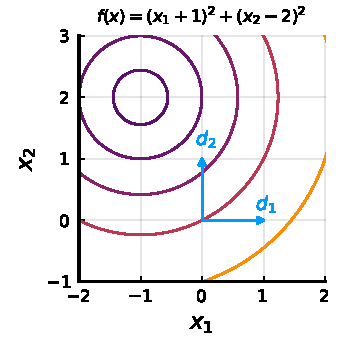
\includegraphics{part_2/chapter_6/figures/orthogonal.pdf}
	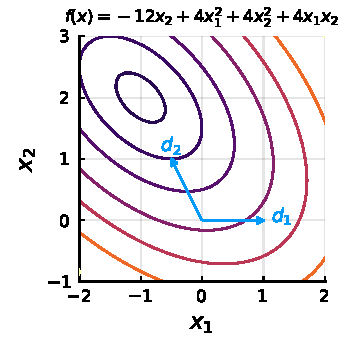
\includegraphics{part_2/chapter_6/figures/H-orthogonal.pdf}
	\caption{$d_1$ and $d_2$ are $H$-conjugates; on the left, $H = I$.} \label{fig:conjugates}
\end{figure}


One can use $H$-conjugate directions to find optimal solutions for the quadratic function $f(x) = c^\top x + \frac{1}{2}x^\top Hx$, where $H$ is a symmetric matrix. Suppose we know directions $d_1, \dots, d_n$ that are $H$-conjugate. Then, given an initial point $x_0$, any point $x$ can be described as $x = x_0 + \sum_{j=1}^n \lambda_jd_j$.

We can then reformulate $f(x)$ as a function of the step size $\lambda$, i.e.,
% 
\begin{flalign*}
f(x) &= F(\lambda) = c^\top (x_0 + \sum_{j=1}^n\lambda_jd_j) + \frac{1}{2}(x_0 + \sum_{j=1}^n\lambda_jd_j) ^\top H (x_0 + \sum_{j=1}^n\lambda_jd_j) \\
&= \sum_{j=1}^n\big{[} c^\top (x_0 + \lambda_j d_j) + \frac{1}{2}(x_0 + \lambda_j d_j) ^\top H (x_0 + \lambda_jd_j)\big{]}.
\end{flalign*}
% 
This reformulation exposes an important properties that having conjugate directions $d_1,\dots, d_n$ allows us to explore: separability. Notice that $F(\lambda) = \sum_{j=1}^n F_j(\lambda_j)$, where $F_j(\lambda_j)$ is given by
%
\begin{align*}
	F_j(\lambda_j) = c^\top (x_0 + \lambda_j d_j) + \frac{1}{2}(x_0 + \lambda_j d_j) ^\top H (x_0 + \lambda_jd_j),
\end{align*}
%
and is, ultimately, a consequence of the linear independence of the conjugate directions. Assuming that $H$ is positive definite, and thus that first-order conditions are necessary and sufficient for optimality, we can then calculate optimal $\overline{\lambda}_j$ for $j=1,\dots, n$ as
\begin{align*}
	F'_j(\lambda_j) & = 0 \\
	c^\top d_j + x_0^\top Hd_j + \lambda_jd_j^\top Hd_j & = 0 \\
	\overline{\lambda}_j & = - \frac{c^\top d_j + x_0^\top Hd_j}{d_j^\top Hd_j}, \text{ for all } j = 1,\dots,n.
\end{align*}
%
This result can be used to devise an iterative method that can obtain optimal solution for quadratic functions in exactly $n$ iterations. From an initial point $x_0$ and a collection of $H$-conjugate directions $d_1, \dots, d_n$, the method consists of the successively executing the following step
%
\begin{align*}
	x_k = x_{k-1} + \lambda_k d_k, \text{ where } \ \lambda_k = - \frac{c^\top d_k + x_{k-1}^\top Hd_k}{d_k^\top Hd_k} 	
\end{align*}
%
Notice the resemblance this method hold with the coordinate descent method. In case $H = I$, then the coordinate directions given by $d_i = 1$ and $d_{j\neq i} = 0$ are $H$-conjugate and thus, the coordinate descent method converges in two iterations. Figure \ref{fig:coord_conjugate} illustrates this behaviour. Notice that, on the left, the conjugate method converges in exactly two iterations, while coordinate descent takes several steps before finding the minimum. On the right, both methods become equivalent, since, when $H = I$, the coordinate directions become also conjugate to each other.
 
\begin{figure}
	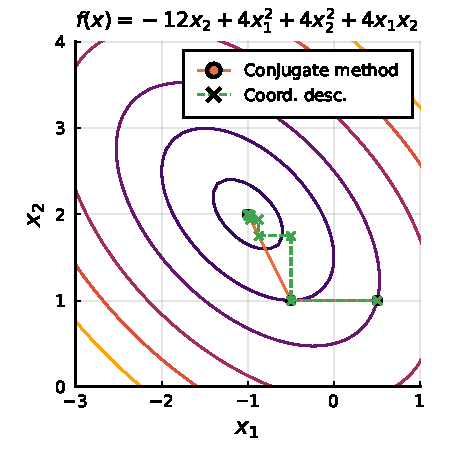
\includegraphics[width=0.48\textwidth]{part_2/chapter_6/figures/coord_conj_H.pdf}
	\hfill
	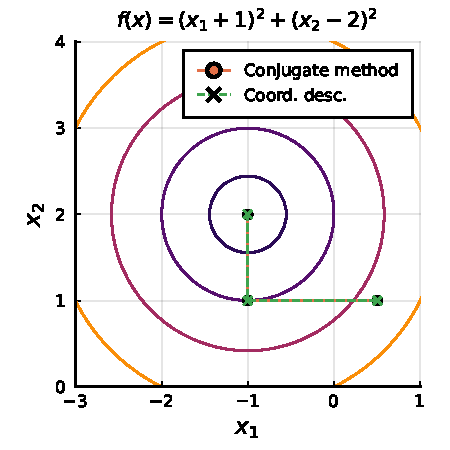
\includegraphics[width=0.48\textwidth]{part_2/chapter_6/figures/coord_conj_I.pdf}
	\caption{Optimising $f$ with the conjugate method and coordinate descent (left). For $H=I$, both methods coincide (right)} \label{fig:coord_conjugate}
\end{figure}


  
\subsubsection{Generating conjugate directions}

The missing part at this point is how one can generate $H$-conjugate directions. This can be done efficiently using an adaptation of the \emph{Gram-Schmidt} procedure, typically employed to generate orthonormal bases. 

We intend to build a collection of conjugate directions $d_0, \dots, d_{n-1}$, which can be achieved provided that we have a collection of linearly independent vectors $\xi_0,\dots,\xi_{n-1}$.

The method proceed as follows. 

\begin{enumerate}
	\item First, set $d_0 = \xi_0$ as a starting step.
	\item At a given iteration $k+1$, we need to set the coefficients $\alpha_{k+1}^i$ such that $d_{k+1}$ is $H$-conjugate to $d_0,\dots,d_k$ and formed by adding $\xi_{k+1}$ to a linear combination of $d_0, \dots, d_{k}$, that is
	$$d_{k+1} = \xi_{k+1} + \sum_{l=0}^k \alpha_{k+1}^l d_l.$$
	\item To obtain $H$-conjugacy one must observe that, for each $i = 0, \dots, k$, 
	\begin{align*}
		{d_{k+1}}^\top H d_i = {\xi_{k+1}}^\top Hd_i + \left(\sum_{l=0}^k \alpha_{k+1}^l d_l \right)^\top Hd_i=0.  
	\end{align*}
	Due to the $H$-conjugacy, $d_l^\top Hd_k = 0$ for all $l \neq k$. Thus the value of $\alpha_{k+1}$ is
	\begin{align}	
		\alpha_{k+1}^i = \frac{-\xi_{k+1}^\top H d_i}{d_i^\top Hd_i}, \text{ for } i = 0,\dots, k. \label{eq:GS_weight}		
	\end{align}

\end{enumerate}

\subsubsection{Gradients and conjugate directions}

The next piece required for developing a method that could exploit conjugacy is the definition of what collection of linearly independent vectors $\xi_0,\dots,\xi_{n-1}$ could be used to generate conjugate directions. In the setting of developing an unconstrained optimisation method, the gradients $\nabla f(x_k)$ can play this part, which is the key result in Theorem \ref{thm:conj_prop}.

\begin{theorem} \label{thm:conj_prop}
Let $f(x) = c^\top x + \frac{1}{2} x^\top Hx$, where H is an  $n\times n$ symmetric matrix. Let $d_1, \dots, d_n$ be H-conjugate, and let $x_0$ be an arbitrary starting point. Let $\lambda_j$ be the optimal solution to $F_j(\lambda_j) = f(x_0 + \lambda_jd_j)$ for all $j = 1,\dots,n$. Then, for $k=1,\dots,n$ we must have:
\begin{enumerate}
\item $x_{k+1}$ is optimal to $\mini\braces{f(x) : x-x_0 \in L(d_1,\dots,d_k)}$ where \lb $L(d_1,\dots,d_k)=\braces{\sum_{j=1}^k \mu_jd_j : \mu_j \in \reals, j = 1,\dots,k}$;
\item $\nabla f(x_{k+1})^\top d_j = 0$, for all $j=1,\dots,k$;
%\item $\nabla f(x_0)^\top d_k = \nabla f(x_k)^\top d_k$.
\end{enumerate}
\end{theorem}

The proof of this theorem is based on the idea that, for a given collection of conjugate directions $d_0,\dots, d_k$, $x_k$ will be optimal in the space spanned by the conjugate directions $d_0, \dots, d_k$, meaning that the partial derivatives of $F(\lambda)$ for these directions is zero. This phenomena is sometimes called \emph{the expanding manifold property}, since at each iteration $L(d_0,\dots,d_k)$ expands in one independent (conjugate) direction at the time. To verify the second point, notice that the optimality condition for $\lambda_j \in \arg\min \braces{F_j(\lambda_j)} $ is $d_j^\top\nabla f(x_0 + \lambda d_j) = 0$.

\subsubsection{Conjugate gradient method}

We have now all parts required for describing the \emph{conjugate gradient method}. The method uses the gradients $\nabla f(x_k)$ as linearly independent vectors to generate conjugate directions, which are then used as search directions $d_k$.

In specific, the method operates generating a sequence of iterates
%
\begin{align*}
	x_{k+1} = x_k + \lambda_k d_k,	
\end{align*}
%
where $d_0 = -\nabla f(x_0)$. Given a current iterate $x_{k+1}$ with $-\nabla f (x_{k+1}) \neq 0$, we use Gram-Schmidth procedure, in particular \eqref{eq:GS_weight}, to generate a conjugate direction $d_{k+1}$ by making the linearly independent vector $\xi_{k+1} = \nabla f(x_{k+1})$. Thus, we obtain
%
\begin{align}
d_{k+1} = -\nabla f(x_{k+1}) + \alpha_kd_k, \text{ with } \alpha_k = \frac{\nabla f(x_{k+1})^\top H d_k}{d_k^\top Hd_k}. \label{eq:conj_grad}
\end{align}
%
Notice that, since $\nabla f(x_{k+1}) - \nabla f(x_k) = H(x_{k+1} - x_k) = \lambda_k H d_k$ and  $d_k= - \nabla f(x_k) + \alpha_{k-1}d_{k-1}$, $\alpha_k$ can be simplified to be
%
\begin{align*}
	\alpha_k &= \frac{\nabla f(x_{k+1})^\top H d_k}{d_k^\top Hd_k} \\
	&= \frac{\nabla f(x_{k+1})^\top (\nabla f(x_{k+1}) - \nabla f(x_k))}{(- \nabla f(x_k) + \alpha_{k-1}d_{k-1})^\top (\nabla f(x_{k+1}) - \nabla f(x_k))} \\
	&= \frac{||\nabla f(x_{k+1})||^2}{||\nabla f(x_k)||^2},
\end{align*}
where the last relation follows from Theorem \ref{thm:conj_prop}. Algorithm \ref{Alg2} summarises the conjugate gradient method. % TODO: Figure out how to explain that \nabla f(x_{k+1})\dot \nabla f(x_k) = 0.

\begin{algorithm}[H]
\caption{Conjugate gradient method} \label{Alg2}
\begin{algorithmic}[1] %line numbering frequency. 
\State {\bf initialise.} tolerance $\epsilon > 0,$ initial point $x_0,$ direction $d_0 = - \nabla f(x_0),$ $k = 1$ 
\While {$||\nabla f(x_k)|| > \epsilon$} 
	\State $y_0 = x_{k-1}$
	\State $d_0 = -\nabla f(y_0)$
    \For {$j = 1,\dots, n$} \label{alg:conj_restart}      
        \State $\overline{\lambda}_j = \argmin_{\lambda \geq 0}\braces{f(y_{j-1} + \lambda d_{j-1})}$
        \State $y_{j} = y_{j-1} + \overline{\lambda}_j d_{j-1}$
        \State $d_{j} = -\nabla f(y_{j}) + \alpha_jd_{j-1}$, where $\alpha_j = \frac{||\nabla f(y_{j})||^2}{||\nabla f(y_{j-1})||^2}$.
    \EndFor
    \State $x_k = y_n$, $k = k+1$
\EndWhile
\State {\bf return} $x_k$.
\end{algorithmic}
\end{algorithm}

The conjugate gradient method using $\alpha_k = \frac{||\nabla f(x_{k+1})||^2}{||\nabla f(x_k)||^2}$ is due to Fletcher and Reeves. %TODO: citation
	An alternative version of the method uses
	%
	\begin{align*}
		\alpha_k = \frac{\nabla f(x_{k+1})^\top (\nabla f(x_{k+1}) - \nabla f(x_k))}{||\nabla f(x_k)||},
	\end{align*}
	%
	which is known for having better numerical properties for solving  problems that are not quadratic.
	
Figure \ref{fig:conjugate_gradient} illustrates the behaviour of the conjugate gradient method when applied to solve $f(x)=e^{(-(x_1-3)/2)} + e^{((4x_2 + x_1)/10)} + e^{((-4x_2 + x_1)/10)}$ using both exact and inexact line searches. 
%
\begin{figure}
	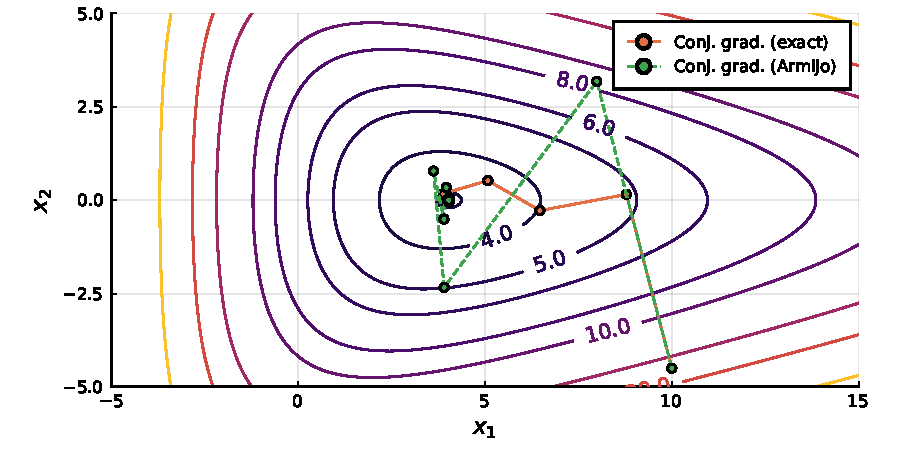
\includegraphics[width=\textwidth]{part_2/chapter_6/figures/conjugate_gradient.pdf}
	\caption{Conjugate gradient method applied to $f$. Convergence is observed in 24 steps using exact line search and 28 using Armijo's rule ($\epsilon = 10^{-6}$)} \label{fig:conjugate_gradient}	
\end{figure}

If $f: \reals^n \mapsto \reals$ is a quadratic function, then the method is guaranteed to converge in exactly $n$ iterations. However, the method can be applied to any differentiable function $f$, in which setting the method behaves as successively solving quadratic approximations of $f$, in a similar fashion to that of Newton's method, but without requiring second-order (Hessian) information, which is the most demanding aspect associated with Newton's method. When employed to non-quadratic functions, the process of obtaining conjugate directions is restarted at the current point $x_k$ after $n$ steps (represented in the loop staring in Line \ref{alg:conj_restart} in Algorithm \ref{Alg2}).

Equation \eqref{eq:conj_grad} exposes an important property of the conjugate gradient method. In general, the employment of second-order terms is helpful for the optimisation method because it encodes \emph{curvature information} on the definition of the search direction. The conjugate gradient method is also capable of encoding curvature information, not by using Hessians, but by weighting the current direction (given by the gradient) $-\nabla f(x_{k+1})$ and the previous direction $\alpha_kd_k$, which naturally compensates for the curvature encoded in the original matrix $H$ (which is the Hessian of the quadratic approximation).


\subsection{Quasi Newton: BFGS method}


\emph{Quasi-Newton methods} is a term referring to methods that use approximations for the inverse of the Hessian of $f$ at $\overline{x}$, $H^{-1}(\overline{x})$, that do not explicitly require second-order information (i.e., Hessians) neither expensive inversion operations. 

In quasi-Newton methods, we consider the search direction $d_k = -D_k \nabla f(x_k)$, where $D_k$ acts as the approximation for the inverse Hessian $H^{-1}(\overline{x})$. To compute $D_k$, we use local curvature information, in the attempt to approximate second-order derivatives. For that, let us define the terms
%
\begin{align*}
&p_k = \lambda_k d_k = x_{k+1} - x_k\\
&q_k = \nabla f(x_{k+1}) - \nabla f(x_k) = H(x_{k+1} - x_k) = Hp_k.
\end{align*}
%
Starting from an initial guess $D_0$, quasi-Newton methods progress by successively updating $D_{k+1} = D_k + C_k$, with $C_k$ being such that it only uses the information in $p_k$ and $q_k$ and that, after $n$ updates, $D_n$ converges to $H^{-1}$.

For that to be the case, we require that $p_j$, $j = 1, \dots, k$ are eigenvectors of $D_{k+1}H$ with unit eigenvalue, that is
%
\begin{align}
		& D_{k+1}Hp_j = p_j, \text{ for } j=1, \dots, k. \label{eq:BFGS_cond1}
\end{align}
%
This condition guarantees that, at the last iteration, $D_n = H^{-1}$. To see that, first, notice the following from \eqref{eq:BFGS_cond1}.
%
\begin{align*}
	& D_{k+1}Hp_j = p_j, \ j = 1,\dots,k \\
	& D_{k+1}q_j = p_j,\ j = 1,\dots,k \\
	& D_kq_j + C_kq_j = p_j \ j = 1,\dots,k \\
	& p_j = D_kHp_j + C_kq_j = p_j + C_kq_j,\ j = 1,\dots,k-1,
\end{align*}
%
which implies that $C_kq_j = 0$ for $j=1,\dots,k-1$. 

Now, for $j = k$, we require that 
%
\begin{align*}
	& D_{k+1} q_k  = p_k \\
	& D_k q_k + C_k q_k  = p_k \\
	& (D_k + C_k) q_k = p_k 
\end{align*}
%
This last condition allows, after $n$ iterations, to recover 
\begin{align}
	D_n = [p_0, \dots, p_{n-1}][q_0, \dots, q_{n-1}]^{-1} = H(x_n) 	\label{eq:BFGS_cond2}
\end{align}

Condition \eqref{eq:BFGS_cond2} is called the \emph{secant condition} as a reference to the approximation to the second-order derivative. Another way of understanding the role this condition has is by noticing the following.
\begin{align}
	D_{k+1} q_k  = p_k \nonumber \\
	D_{k+1}(\nabla f(x_{k+1}) - \nabla f(x_k)) = x_{k+1} - x_k \nonumber \\
	\nabla f(x_{k+1}) = \nabla f(x_k) + D_{k+1}^{-1}(x_{k+1} - x_k) \label{eq:bfgs_cond_explain}, 
\end{align}
%
where $D_{k+1}^{-1}$ can be seen as an approximation to the Hessian $H$, just as $D_{k+1}$ is an approximation to $H^{-1}$. Now, consider the second-order approximation of $f$ at $x_k$
\begin{align*}
	q(x) = f(x_k) + \nabla f(x_k)^\top(x -x_k) + \frac{1}{2}(x - x_k)^\top H(x_k)(x - x_k). 	
\end{align*}
We can now notice the resemblance the condition \eqref{eq:bfgs_cond_explain} holds with
%
\begin{align*}
	\nabla q(x) = \nabla f(x_k) + H(x_k)^\top(x - x_k) = 0.	
\end{align*}
% 
In other words, at each iteration, the updates are made such that the optimality conditions in terms of the quadratic expansion remains valid. 

The \emph{Davidon-Fletcher-Powell} (DFP) is one classical quasi-Newton method available. It employs updates of the form
%
\begin{align*}
D_{k+1} = D_k + C^{DFP} = D_{k} + \frac{p_kp_k^\top}{p_k^\top q_k} - \frac{D_kq_kq_k^\top D_k}{q_k^\top D_kq_k} 	
\end{align*}
%
We can verify that $C^{DFP}$ satisfies conditions \eqref{eq:BFGS_cond1} and \eqref{eq:BFGS_cond2}. For that, notice that
\begin{enumerate}
	\item[(1)] $C^{DFP}q_j = C^{DFP}Hp_j$
\item[]\hspace{38pt}$=\frac{p_kp_k^\top Hp_j}{p_k^\top q_k} - \frac{D_kq_kp_k^\top H D_kHp_j}{q_k^\top D_kq_k} = 0, \ \text{ for }j=1,\dots,k-1$;
\item[(2)] $C^{DFP}q_k \hspace{-1.5pt}= \frac{p_kp_k^\top q_k}{p_k^\top q_k} - \frac{D_kq_kq_k^\top D_kq_k}{q_k^\top D_kq_k} = p_k - D_kq_k$.
\end{enumerate} 
%
The main difference between available quasi-Newton methods is the nature of the matrix $C$ employed in the updates. Over the years, several ideas emerged in terms of generating updates that satisfied the above properties. The most widely used quasi-Newton method is the \emph{Broyden-Fletcher-Goldfarb-Shanno} (BFGS), which has been widely shown to have remarkable practical performance. BFGS is part of the Broyden family of updates, given by
%
\begin{align*}
C^B = C^{DFP} + \phi \frac{\tau_j v_kv_k^\top}{p_k^\top q_k},  	
\end{align*}
%
where $v_k = p_k - \left(\frac{1}{\tau_k}\right)D_kq_k$, $\tau_k = \frac{q_j^\top D_kq_k}{p_k^\top q_k}$, and $\phi \in (0,1)$. The extra term in the Broyden family of updates is designed to help with mitigating numerical difficulties from near-singular approximations.

It can be shown that all updates from the Broyden family also satisfy the quasi-Newton conditions \eqref{eq:BFGS_cond1} and \eqref{eq:BFGS_cond2}. The BFGS update is obtained for $\phi = 1$, which renders
\begin{align*}
	C^{BFGS}_k = \frac{p_kp_k^\top}{p_k^\top q_k}\left(1 + \frac{q_k^\top D_kq_k}{p_k^\top q_k}\right) - \frac{D_kq_kp_k^\top + p_kq_k^\top D_k}{p_k^\top q_k}.
\end{align*}

The BFGS method is often presented explicitly approximating the Hessian $H$ instead of its inverse, which is useful when using specialised linear algebra packages that rely on the ``backslash'' operator to solve linear systems of equations. Let $B_k$ be the current approximation of $H$. Then $D_{k+1} = B^{-1}_{k+1} = (B_k + \overline{C}_k^{BFGS})^{-1}$, with
%
\begin{align*}
\overline{C}_k^{BFGS} = \frac{q_kq_k^\top}{q^\top_kp_k} - \frac{B_kp_kp_k^\top B_k}{p_k^\top B_kp_k}.
\end{align*}
% 
The update for the inverse Hessian $H^{-1}$ can then be obtained using the \emph{Sherman-Morrison formula}.

Figure \ref{fig:BFGS} illustrates the behaviour of the BFGS method when applied to solve 
$$
f(x)=e^{(-(x_1-3)/2)} + e^{((4x_2 + x_1)/10)} + e^{((-4x_2 + x_1)/10)}
$$ 
using both exact and inexact line searches. Notice how the combination of imprecisions both in the calculation of $H^{-1}$ and in the line search turns the search noisy. This combination (BFGS combined with Armijo rule) is, however, widely used in efficient implementations of several nonlinear optimisation methods.

\begin{figure}
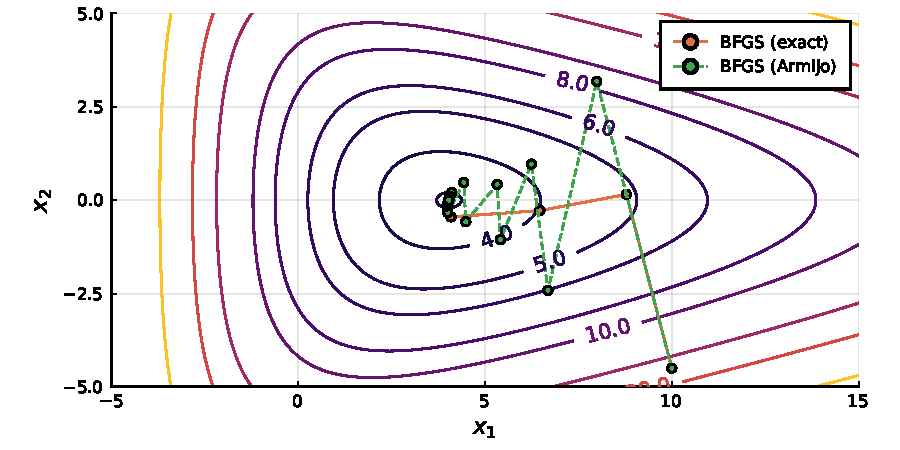
\includegraphics[width=\textwidth]{part_2/chapter_6/figures/bfgs.pdf}
\caption{BFGS method applied to $f$. Convergence is observed in 11 steps	using exact line search and 36 using Armijo's rule ($\epsilon = 10^{-6}$)} \label{fig:BFGS}	
\end{figure}



A variant of BFGS, called the \emph{limited memory} BFGS (l-BFGS) utilises  efficient implementations that do not require storing the whole approximation for the Hessian, but only a few most recent $p_k$ and $q_k$ vectors.


\section{Complexity, convergence and conditioning}

Several aspects must be considered when analysing the performance of algorithms under a given setting and, in each, a multitude of theoretical results that can be used to understand, even if to some extent, the performance of a given optimisation method.

We focus on three key properties that one should be aware when employing the methods we have seen to solve optimisation problems. The first two, \emph{complexity} and \emph{convergence} refer to the algorithm itself, but often involve considerations related to the function being optimised. \emph{Conditioning}, on the other hand, is a characteristic exclusively related to the problem at hand. Knowing how the ``three C's'' can influence the performance of an optimisation problem is central in making good choices in terms of which optimisation method to employ. 


\subsection{Complexity}

\emph{Algorithm complexity analysis} is a discipline from computer science that focus on deriving worst-case guarantees in terms of the number of computational steps required for an algorithm to converge, given an input of known size. For that, we use the following definition to identify efficient, generally referred to as \emph{polynomial}, algorithms.

\begin{definition}[Polynomial algorithms]
    Given a problem $P$, a problem instance $X \in P$ with length $L(X)$ in binary representation, and an algorithm $A$ that solves $X$, let $f_A(X)$ be the number of \emph{elementary calculations} required to run $A$ on $X$. Then, the running time of $A$ on $X$ is proportional to $$f^*_A(n) = \sup_X\braces{f_A(X) : L(X) = n}.$$ Algorithm $A$ is \emph{polynomial} for a problem $P$ if $f^*_A(n) = O(n^p)$ for some integer $p$.
\end{definition}

Notice that this sort of analysis only render bounds on the worst-case performance. Though it can be informative under a general setting, there are several well known examples in that experimental practice does not correlate with the complexity analysis. One famous example is the simplex method for linear optimisation problems, which despite not being a polynomial algorithm, presents widely-demonstrated reliable (polynomial-like) performance. 

\subsection{Convergence}

In the context of optimisation, \emph{local analysis} is typically more informative regarding to the behaviour of optimisation methods. This analysis tend to disregard initial steps further from the initial points and concentrate on the behaviour of the sequence $\braces{x_k}$ to a unique point $\overline{x}$.

The convergence is analysed by means of \emph{rates of convergence} associated with \emph{error functions} $e: \reals^n \mapsto \reals$ such that $e(x) \geq 0$. Typical choices for $e$ include:
\begin{itemize}
\item $e(x) = ||x - \overline{x}||$;
\item $e(x) = |f(x) - f(\overline{x})|$.
\end{itemize}

The sequence $\braces{e(x_k)}$ is then compared to the geometric progression $\beta^k$, with $k=1,2,\dots,$ and $\beta \in (0,1)$. We say that a method presents \emph{linear convergence} if exists $q > 0$ and $\beta \in (0,1)$ such that $e(x) \leq q\beta^k$ for all $k$. An alternative way of posing this result is stating that
%
\begin{align*}
	\lim_{k\rightarrow\infty} \sup \frac{e(x_{k+1})}{e(x_k)} \leq \beta.
\end{align*}
%
We say that an optimisation method converges superlinearly if the rate of convergence tends to zero. That is, if exists $\beta \in (0,1)$, $q > 0$ and $p > 1$ such that $e(x_k) \leq q\beta^{p^k}$ for all $k$. For $k=2$, we say that the method presents quadratic convergence. Any $p$-order convergence is obtained if 
%
\begin{align*}
	\lim_{k\rightarrow\infty} \sup \frac{e(x_{k+1})}{e(x_k)^p} < \infty, \text{ which is true if }
\lim_{k\rightarrow\infty} \sup \frac{e(x_{k+1})}{e(x_k)} = 0	.
\end{align*}

Linear convergence is the most typical convergence rate for nonlinear optimisation methods, which is satisfactory if $\beta$ is not too close to one. Certain methods are capable of achieving superlinear convergence for certain problems, being Newton's method an important example.

In light of what we discussed, let us analyse the convergence rate of some of the methods earlier discussed. We start by posing the convergence of gradient methods.
%
\begin{theorem}[Convergence of the gradient method] \label{thm:gradient_conv}
Let $f(x) = \frac{1}{2}x^\top Hx$ where $H$ is a positive definite symmetric matrix. Suppose $f(x)$ is minimised with the gradient method using an exact line search. Let $\underline{\lambda} = \min_{i=1,\dots,n}\lambda_i$ and $\overline{\lambda} = \max_{i=1,\dots,n}\lambda_i$, where $\lambda_i$ are eigenvalues of $H$. Then, for all $k$,
$$ \frac{f(x_{k+1})}{f(x_k)} \leq \left(\frac{\overline{\lambda}-\underline{\lambda}}{\overline{\lambda}+\underline{\lambda}}\right)^2
$$
\end{theorem}

Theorem \ref{thm:gradient_conv} implies that, under certain assumptions, the gradient methods present \emph{linear convergence}. Moreover, this result shows that the convergence rate is \emph{dependent} on the scaling of the function, since it depends on the ratio of eigenvalues of $H$, which in turn can be modified by scaling $f$. This results exposes an important shortcoming that gradient methods present: the dependence on the \emph{conditioning} of the problem, which we will discuss shortly. Moreover, this result can be extended to incorporate functions other than quadratic and also inexact line searches. 

The convergence of Newton's method is also of interest since, under specific circumstances, it presents a  quadratic convergence rate. Theorem \ref{thm:newton_convergence} summarises these conditions.

\begin{theorem}[Convergence of Newton's method - general case] \label{thm:newton_convergence}
Let $g: \reals^n \rightarrow \reals^n$ be differentiable, $\overline{x}$ such that $g(\overline{x}) = 0$, and let $\braces{e(x_k)} $ $= \braces{||x_k - \overline{x}||}$. Moreover, let $N_\delta(\overline{x}) = \braces{x : ||x  - \overline{x}|| \leq \delta}$ for some $\delta >0 $. Then
\begin{enumerate}
\item There exists $\delta > 0$ such that if $x_0 \in N_\delta(\overline{x})$, the sequence $\braces{x_k}$ with $x_{k+1} = x_k - (\nabla g(x_k)^\top)^{-1}g(x_k)$ belongs to $N_\delta(\overline{x})$ and converges to $\overline{x}$, while $\braces{e(x_k)}$ converges superlinearly.
\item If for some $L>0$, $M>0$, and for all $x,y$ $\in N_\delta(\overline{x})$, $\lambda \in (0,\delta]$
$$||\nabla g(x) - \nabla g(y)|| \leq L||x-y|| \quad\text{and }\quad ||(\nabla g(x_k)^\top)^{-1}|| \leq M,$$ 
then, if $x_0 \in N_\delta(\overline{x})$, we have for $k = 0,1,\dots$
\vspace{-6pt}
$$ ||x_{k+1} - \overline{x}|| \leq \frac{LM}{2}||x_k - \overline{x}||^2.
\vspace{-6pt}
$$
If $\frac{LM\delta}{2} < 1$ and $x_0 \in N_\delta(\overline{x})$, $\braces{e(x_k)}$ converges quadratically.
\end{enumerate}
\end{theorem}

Notice that the convergence of the method is analysed in two distinct phases. In the first phase, referred to as 'damped' phase, superlinear convergence is observed within the neighbourhood $N_\delta(\overline{x})$ defined by $\delta$. The second phase is where quadratic convergence is observed and it happens when $\delta < \frac{2}{LM}$, which in practice can only be interpreted as small enough, as the constants $L$ (the Lipschitz constant) and $M$ (a finite bound for the norm of the Hessian) cannot be easily estimated in practical applications. 

However, it is interesting to notice that the convergence result for Newton's method do not depend  on the scaling of the problem, like the gradient method. This property, called \emph{affine invariance} is one of the greatest features that Newton's method possess. 

Figure \ref{fig:convergence} compare the convergence of four methods presented considering $f(x)=e^{(-(x_1-3)/2)} + e^{((4x_2 + x_1)/10)} + e^{((-4x_2 + x_1)/10)}$, employing exact line search and using $e(x) = ||x_k - \overline{x}||$. Notice how the quadratic convergence of Newton's method compare with the linear convergence of the gradients method. The other two, conjugate gradients and BFGS, present superlinear convergence.

\begin{figure}
	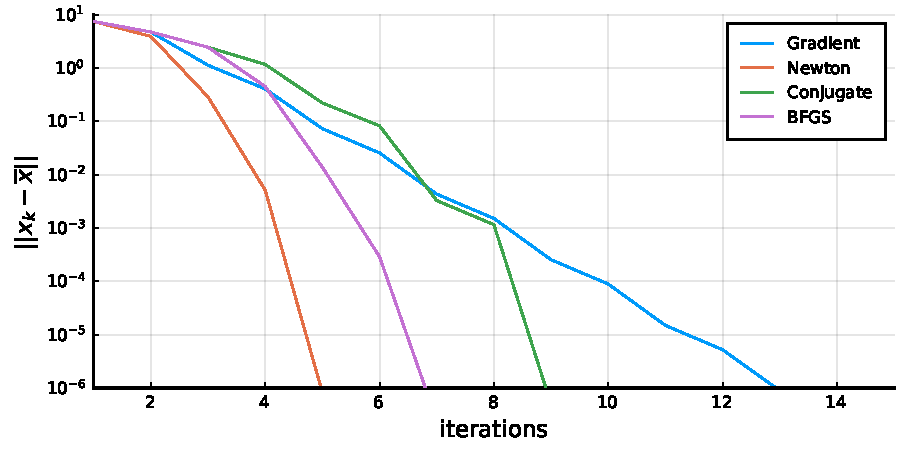
\includegraphics[width=0.8\textwidth]{part_2/chapter_6/figures/convergence.pdf}
	\caption{Convergence comparison for the four methods}\label{fig:convergence}
\end{figure}


\subsection{Conditioning}

The \emph{condition number} of a symmetric matrix is given by 
\begin{align*}
	\kappa = ||A||_2 ||A^{-1}||_2 = \frac{\max_{i = 1,\dots,n} \braces{\lambda_i}}{\min_{i = 1,\dots,n} \braces{\lambda_i}} = \frac{\overline{\lambda}}{\underline{\lambda}}	
\end{align*}

The condition number $\kappa$ is an important measure in optimisation, since it can be used to predict how badly scaled a problem might be. Large $\kappa$ values mean that numerical errors will be amplified after repeated iterations, in particular matrix inversions.

Roughly speaking, having $\kappa \geq 10^k$ means that at each iteration, $k$ digits of accuracy are lost. As general rule, one would prefer smaller $\kappa$ numbers, but good values are entirely problem dependent. 

One way of understanding the role that the conditioning number $\kappa$ has is to think the role that the eigenvalues of the Hessian have in the shape of the level curves of quadratic approximations of a general function $f : \reals^n \mapsto \reals$. First, let us consider the Hessian $H(x)$ at a given point $x \in \reals^n$ is the identity matrix $I$, for which all eigenvalues are 1 and eigenvectors are $e_i$, $i = 1, \dots, n$, where $e_i$ is the vector with component 1 in the position $i$ and zero everywhere else. This means that in the direction of the $n$-eigenvectors, the ellipsoid formed by the level curves (specifically, the lower level sets) of $f$ stretch by the same magnitude and, therefore, the level curves of the quadratic approximation are in fact a circle. Now, suppose that for one of the dimensions $i$ of the matrix $H(x)$, we have one of the eigenvalues greater than 1. What we would see is that the level curves of the quadratic approximation will be more stretched in that dimension $i$ than in the others. The reason for that is because the Hessian plays a role akin to that of a characteristic matrix in an ellipsoid (specifically due to the second order term $\frac{1}{2}(x - x_k)^\top H(x_k)(x - x_k)$ in the quadratic approximation). 

Thus, larger $\kappa$ will mean that the ratio between the eigenvalues is larger, which in turn implies that there is eccentricity in the lower level sets (i.e., the lower level sets are far wider in one direction than in others), which ultimately implies that first-order methods struggle since often the gradients often point to directions that only show descent for small step sizes.

\begin{figure}[h]
\begin{subfigure}[b]{\textwidth}
    \centering
   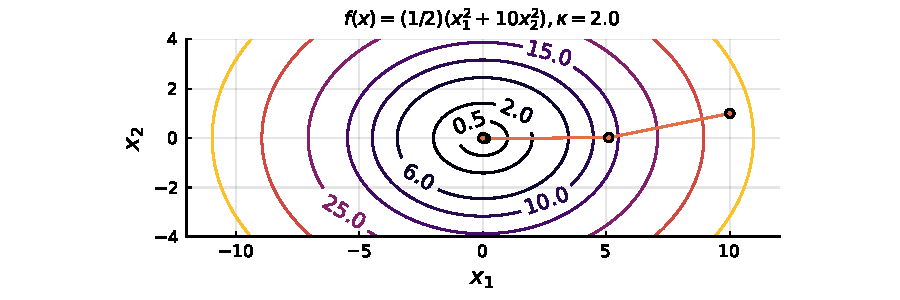
\includegraphics[width=\textwidth]{part_2/chapter_6/figures/gradient_k2.pdf}
\end{subfigure}
\hfill
\begin{subfigure}[b]{\textwidth}
    \centering
   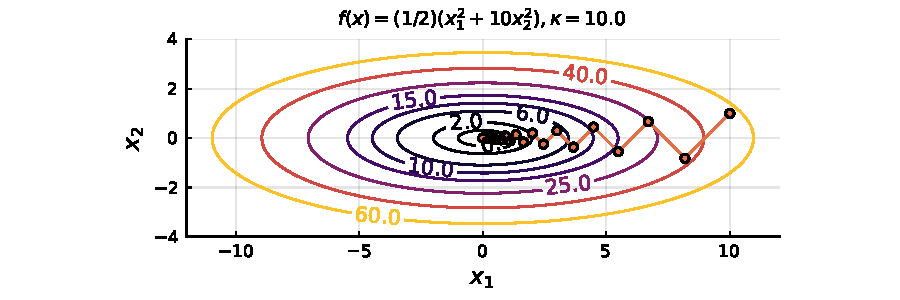
\includegraphics[width=\textwidth]{part_2/chapter_6/figures/gradient_k10.pdf}
\end{subfigure}
\caption{The gradient method with exact line search for different $\kappa$.}\label{fig:figure_5}
\end{figure}



Figure \ref{fig:figure_5} illustrates the effect of different condition numbers on the performance of the gradient method. As can be seen, the method require more iterations for higher conditioning numbers, in accordance to the convergence result presented in Theorem \ref{thm:gradient_conv}.

